\subsection{Kleinste und grösste positive Zahlen}\label{sec:groesste-kleinste}

Es gibt unendlich viele reelle Zahlen. Wir können aber nur endlich viele davon in einem Fliesskommazahlensystem darstellen. Im Kasten, welcher uns die Mantisse veranschaulicht, finden nur endlich viele Bits Platz. Das Seil, welches den Kasten an den Komma bindet und welches uns den Exponenten veranschaulicht, hat ebenfalls eine endliche Länge.

Weil es endlich viele darstellbare Zahlen gibt, muss es eine kleinste und eine grösste Zahl geben. In diesem Abschnitt werden wir die kleinste und die grösste positive darstellbare Zahlen in Abhängigkeit vom Exponentenbereich und Mantissenlänge finden.


\begin{beispiel}
Wir konstruieren die grösste positive Zahl im Fliesskommazahlensystem mit Mantissenlänge \(5\) und Exponenten von \(-3\) bis \(3\).

In violett wird die reelle Zahl in Basis 2 aufgeschrieben, in der zweiten Zeile kommt die ''Kasten-und-Seil''-Darstellung aus der Einführung, in der dritten Zeile das Bitmuster und als letztes die Exponentialschreibweise. Darstellungsübergreifend ist die Mantisse in braun markiert, der Exponent in Orange und das Vorzeichen in grün.

Als erstes platzieren wir den Kasten. Damit die Zahl so gross wie möglich wird, muss der Kasten links vom Komma stehen, und zwar so weit entfernt wie möglich. Wir haben aber eine Einschränkung: Das Seil muss immer mit dem Komma verbunden bleiben.
\begin{figure}[H]
\centering
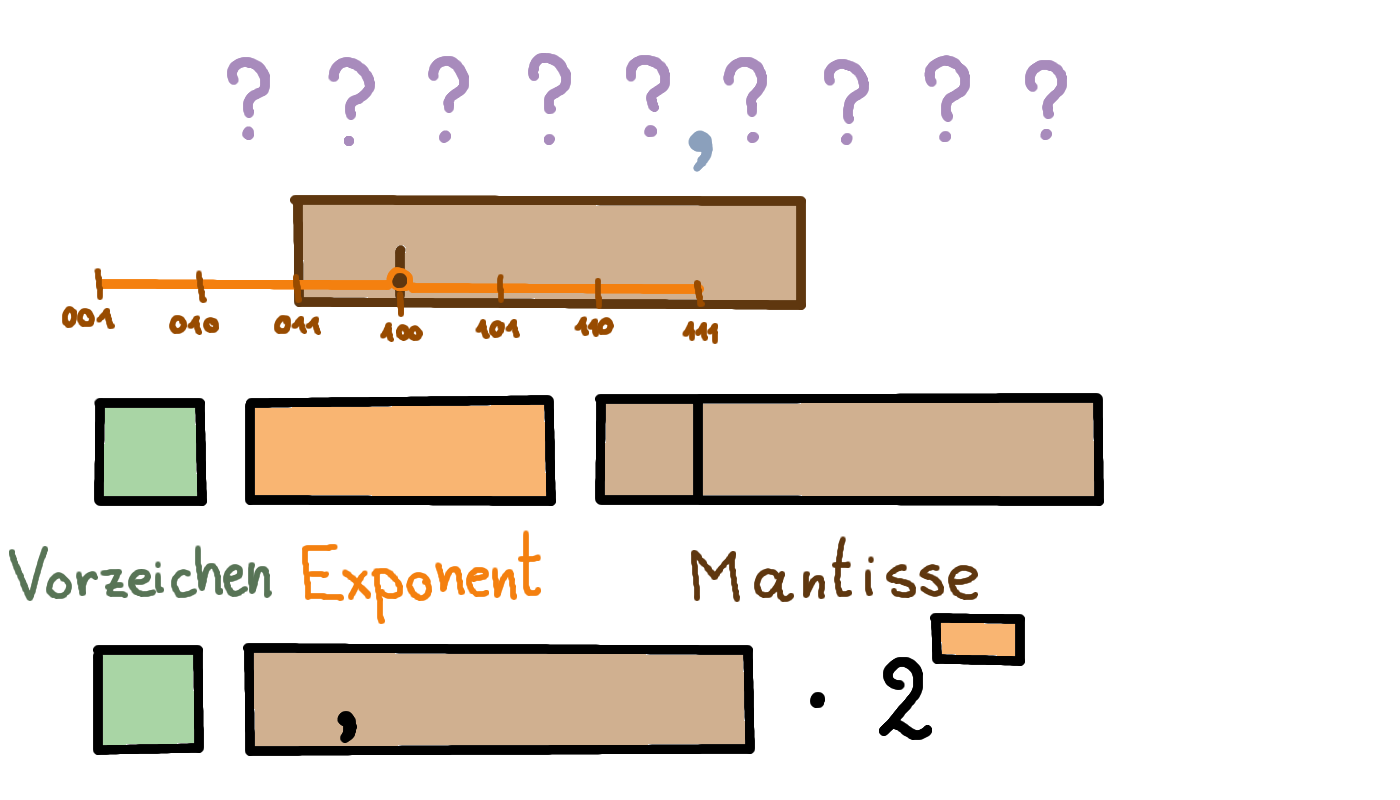
\includegraphics[width=0.85\linewidth]{Pictures/groessteZahl1.png}
\end{figure}
Der Exponent muss also möglichst gross sein.

Was ist mit der Mantisse? Sicher muss eine Eins an der ersten Stelle stehen.
\begin{figure}[H]
\centering
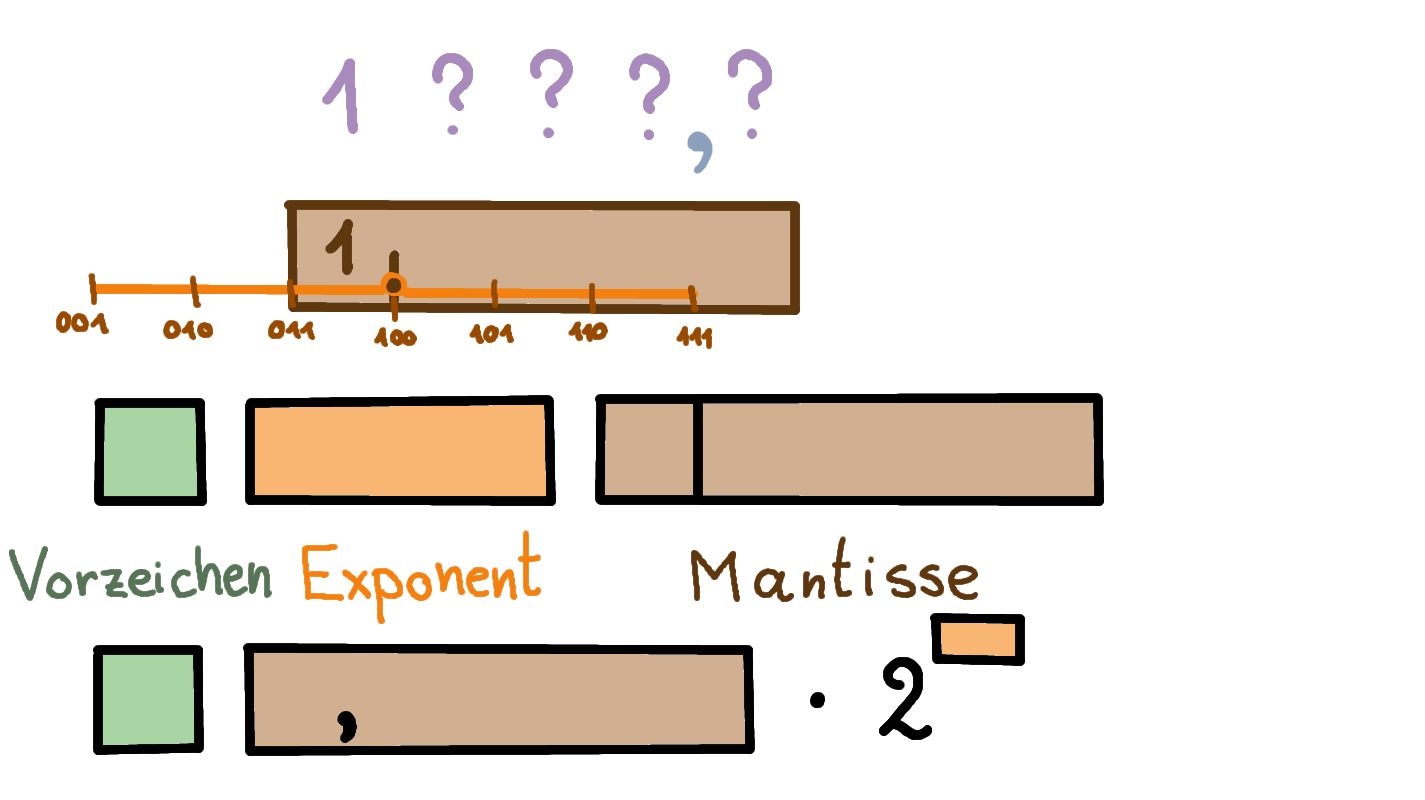
\includegraphics[width=0.85\linewidth]{Pictures/groessteZahl2.png}
\end{figure}

Damit die Mantisse möglichst gross wird, muss sie aus lauter Einser bestehen.
\begin{figure}[H]
\centering
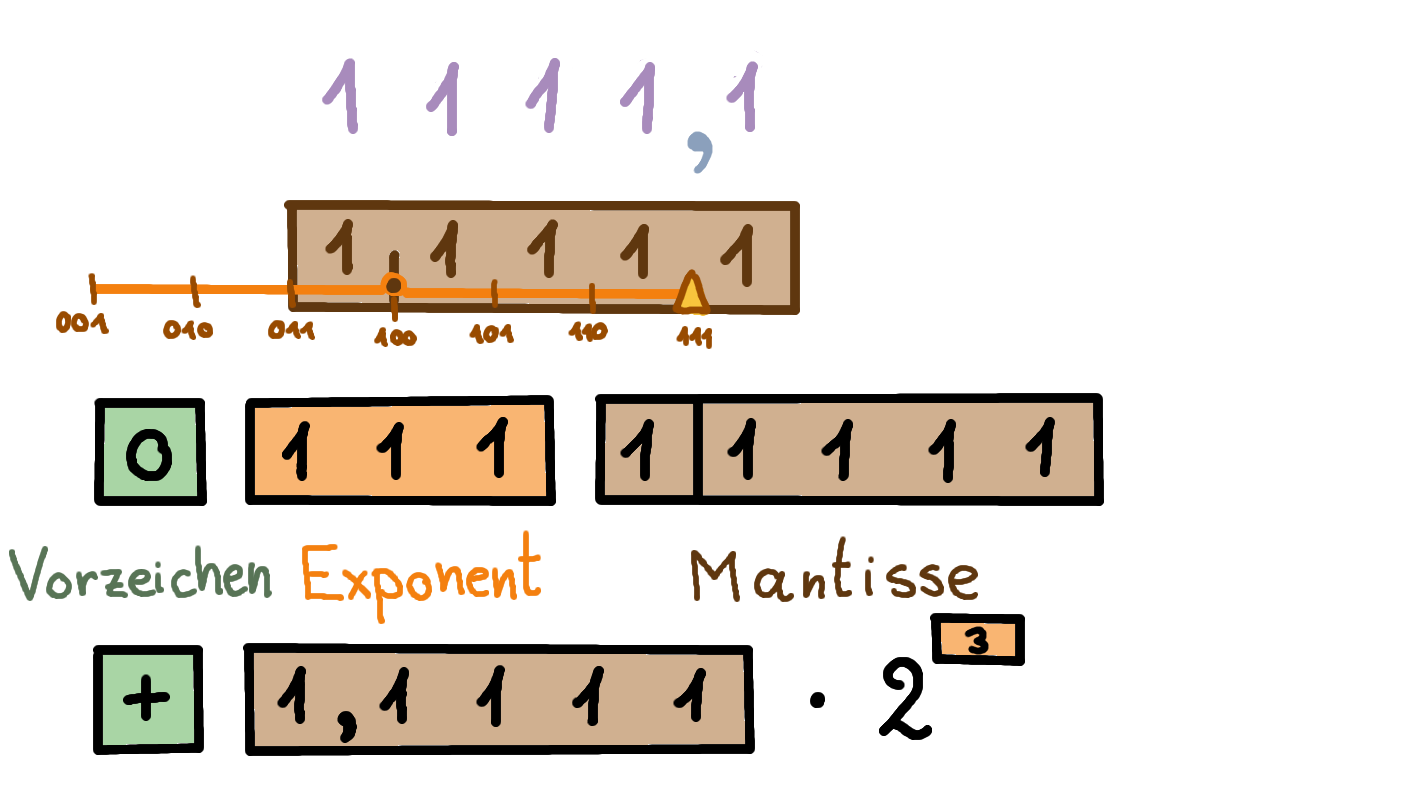
\includegraphics[width=0.85\linewidth]{Pictures/groessteZahl3.png}
\end{figure}

Die grösste darstellbare Zahl in diesem Fliesskommazahlensystem ist also \(15.5\).
\end{beispiel}

\begin{aufgabe}\label{kleinsteZahl-5-3}
Konstruiere die kleinste positive Zahl im Fliesskommazahlensystem mit Mantissenlänge \(5\) und Exponenten von \(-3\) bis \(3\). Schreibe die Zahl im ''Kasten-und-Seil''-Modell, als Bitmuster und in der binären Exponentialschreibweise auf und berechne ihren Dezimalwert.
\end{aufgabe}

Wir haben gesehen, dass die positive Zahlen, welche sich exakt in einem Fliesskommazahlensystem mit Mantissenlänge 5 und 3 Bits für den Exponenten darstellen lassen, zwischen \(1/8\) und \(15.5\) liegen müssen. Wie stark verändern sich diese Werte, wenn wir ein Bit weniger für die Mantisse zur Verfügung stellen?

\begin{aufgabe}\label{groesste-kleinste-4-3}
Betrachte das Fliesskommazahlensystem mit Mantissenlänge \(4\) und Exponenten von \(-3\) bis \(3\). Was erwartest du für die grösste positive darstellabare Zahl? Ist sie kleiner oder grösser als \(15.5\)? Wie stark unterscheidet sie sich davon?

Und was erwartest du für die kleinste positive darstellbare Zahl? Ist sie grösser oder kleiner als \(1/8\)? Wie stark unterscheidet sie sich davon?

Konstruiere die grösste und die kleinste positive darstellbare Zahlen in diesem System.  Schreibe die Zahlen im ''Kasten-und-Seil''-Modell, als Bitmuster und in der binären Exponentialschreibweise auf und berechne den Dezimalwert. 
\end{aufgabe}

In der vorherigen Aufgabe hast du gesehen, welchen Einfluss die Mantissenlänge auf die grösste und kleinste positive darstellbare Zahlen haben. Das Ergebnis könnte überraschend kommen. Da wir ein Bit weniger für die Mantisse und gleich viele Bits für den Exponenten genommen haben, ist unser Bitmuste um ein Bit kürzer geworden und somit können wir höchstens halb so viele Zahlen darstellen als vorher. Trotzdem haben sich die grösste und die kleinste positive darstellbare Zahlen kaum verändert.

Was passiert, wenn wir nun ein Bit weniger für den Exponenten nehmen?

\begin{aufgabe}\label{groesste-kleinste-5-2}
Betrachte das Fliesskommazahlensystem mit Mantissenlänge \(5\) und mit nur \(2\) Bits, um den Exponenten zu kodieren.
\begin{enumerate}[(a)]
\item Welche Exponenten können wir mit \(2\) Bits darstellen? Wie lang wird das Seil? Zeichne das ''Kasten-und-Seil''-Modell für dieses Fliesskommazahlensystem.
\item Was erwartest du für die grösste und die kleinste positive darstellbaren Zahlen? Wie stark unterscheiden sie sich von \(15.5\) und \(1/8\)?
\item Konstruiere die grösste und die kleinste positive darstellbare Zahlen in diesem System.  Schreibe die Zahlen im ''Kasten-und-Seil''-Modell, als Bitmuster und in der binären Exponentialschreibweise auf und berechne den Dezimalwert.
\end{enumerate}
\end{aufgabe}

In der vorherigen Aufgabe hast du gesehen, welchen Einfluss die Länge der Exponentenkodierung auf die grösste und kleinste positive darstellbare Zahlen hat. Wie auch im Fliesskommazahlensystem mit Mantissenlänge \(4\) und \(3\) Bits für den Exponenten, können wir im Fliesskommazahlensystem aus Aufgabe \ref{groesste-kleinste-5-2} höchstens halb so viele Zahlen darstellen wie im Fliesskommazahlensystem mit Mantissenlänge \(5\) und \(3\) Bits für die Exponentenkodierung. Der Bereich der darstellbaren Zahlen hat sich dieses Mal extrem verändert.

\begin{aufgabe}\label{groesste-kleinste-allgemein}
Wie sehen die kleinste und die grösste positive darstellbare Zahlen im allgemeinen Fliesskommazahlensystem aus? Nehme Mantissenlänge \(m\) und Exponent zwischen \(e_{min}\) und \(e_{max}\) an. Schreibe die kleinste und die grösste positive darstellbare Zahl in diesem Fliesskommazahlensystem als Bitmuster und in der binären Exponentialdarstellung auf.
\end{aufgabe}



\subsection{Darstellbare Zahlen}

Wir wissen, dass es eine kleinste und eine grösste positive Zahl gibt, welche sich exakt in einem Fliesskommazahlensystem darstellen lassen. Dass man nicht alle unendlich viele reelle Zahlen zwischen diesen zwei Schranken darstellen kann, können wir uns denken. Die Frage ist nun, welche Zahlen sich darstellen lassen und wie sich der Abstand zwischen darstellbaren Zahlen verhält.

Hier und in den folgenden Kapiteln, falls nicht speziell vermerkt, werden wir mit Mantissenlänge \(5\) und Exponentenbereich von \(-3\) bis \(3\) arbeiten.

\begin{beispiel}
Nehmen wir eine Zahl zwischen 1/8 und 15.5 (die kleinste und grösste positive darstellbare Zahlen in diesem Fliesskommazahlensystem), zum Beispiel \(10.25\). Lässt sich diese Zahl darstellen?

\begin{figure}[H]
\centering
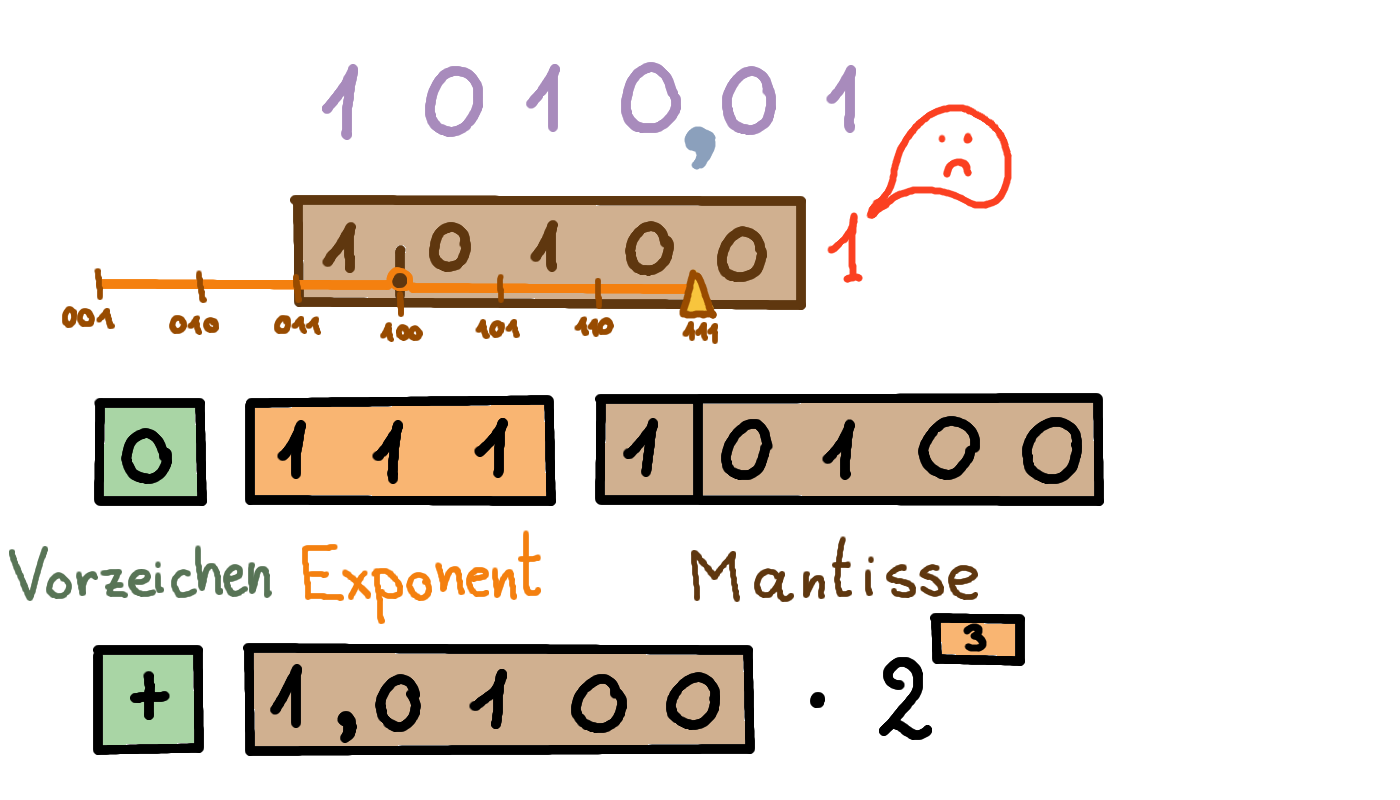
\includegraphics[width=0.75\linewidth]{Pictures/ZahlenDarstellen10-25.png}
\end{figure}

Diese Zahl lässt sich in gegebenem System nicht exakt darstellen. Für die letzte \(1\) gibt es in der Mantisse kein Platz. Deswegen wird \(10.25\) mit \(10.0\) \textbf{approximiert}.
\end{beispiel}

Wir haben gesehen, dass reelle Zahlen sich nur dann exakt darstellen lassen, wenn alle signifikante Stellen in der Mantisse Platz haben.

\begin{beispiel}
Betrachten wir die Zahl \(1\).

In einem Fliesskommazahlensystem lassen sich nur endlich viele Zahlen exakt darstellen. Einige von diesen darstellbaren Zahlen sind grösser als \(1\). Da es nur endlich davon gibt, muss es darunter eine kleinste geben. Diese Zahl bezeichnen wir hier als ''nächste'' oder ''nächstgrösste''. Die ''vorherige'' oder ''nächstkleinste'' darstellbare Zahl ist entsprechend die grösste unter den darstellbaren Zahlen, die kleiner als \(1\) sind.

Wie sieht die nächstgrösste Nachbarzahl von \(1\) aus?

Im ersten Schritt stellen wir die Zahl \(1\) im gegebenem Fliesskommazahlensystem dar.
\begin{figure}[H]
\centering
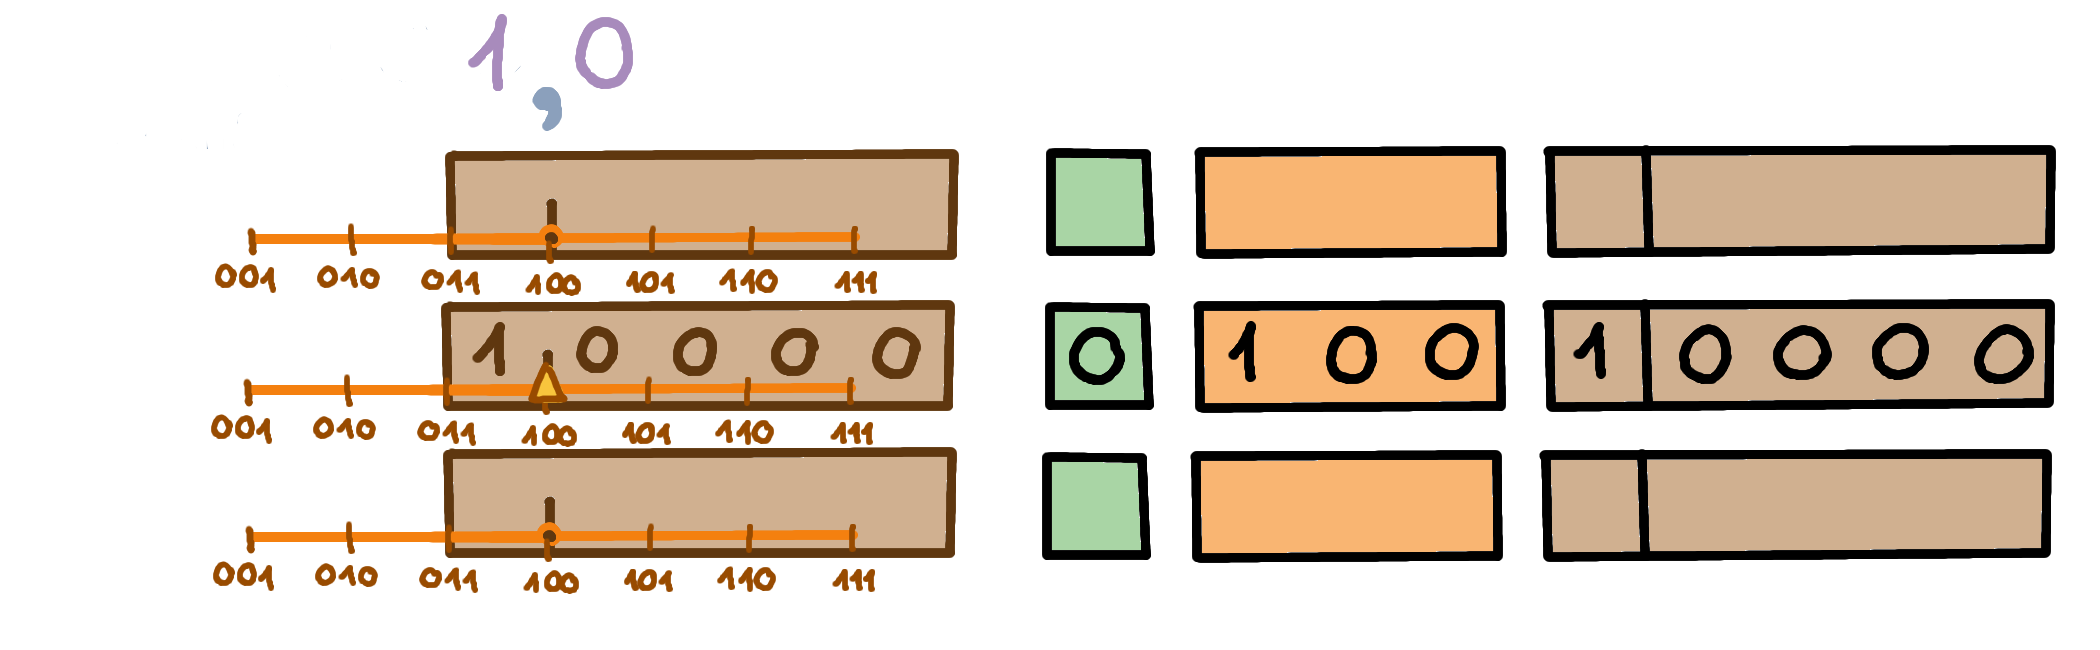
\includegraphics[width=\linewidth]{Pictures/Nachbarn1_1.png} 
\end{figure}

Wir suchen die Zahl, die minimal grösser als \(1\) ist.

Den Exponenten können wir in diesem Fall nicht verändern: Wenn wir den Kasten nach rechts bewegen, dann wird die Zahl kleiner; wenn wir den Kasten nach links bewegen, dann wird die Zahl wegen der obligatorischen führenden Eins zu gross.

Also müssen wir die Mantisse verändern. Da wir eine grössere Zahl suchen, müssen wir eine der Nullen zu einer Eins machen. Welche? Diejenige mit dem kleinsten Wert, d.h. die letzte Eins rechts.

\begin{figure}[H]
\centering
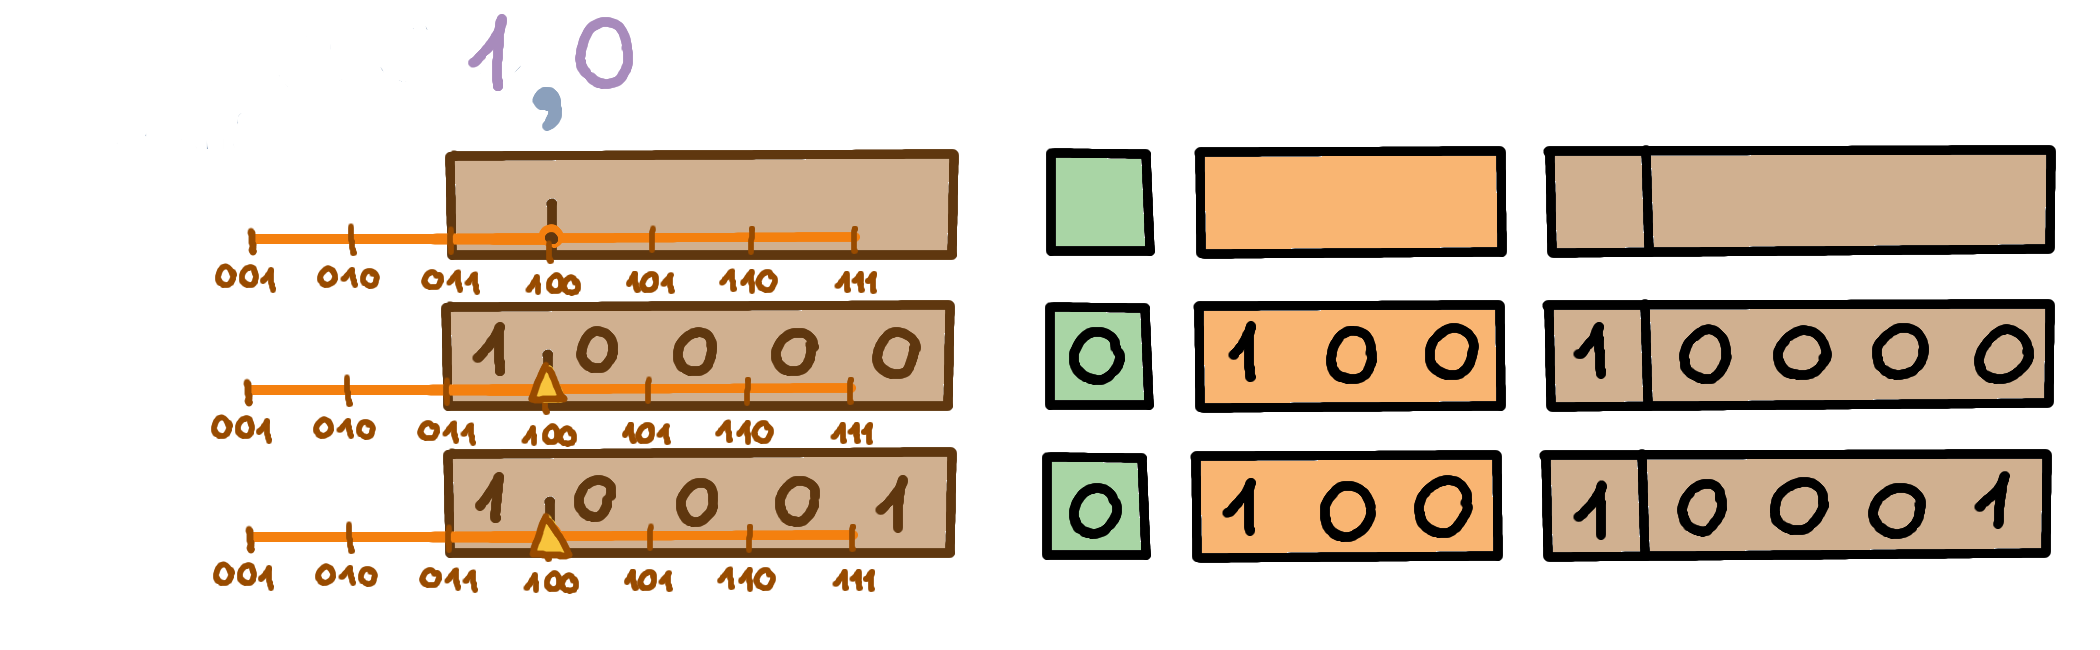
\includegraphics[width=\linewidth]{Pictures/Nachbarn1_N.png} 
\end{figure}
Die nächste darstellbare Zahl ist also \(1 + 1/16 = 17/16\).
\end{beispiel}

\begin{aufgabe}\label{nachbarn-vorherige}
Betrachte die Zahl \(1\). Finde die nächstkleinste darstellbare Zahl. Ist der Abstand zwischen der nächstkleinsten Zahl und \(1\) gleich dem Abstand zwischen \(1\) und der nächstgrössten Zahl?
\end{aufgabe}

\begin{aufgabe}\label{nachbarn}
Finde die nächste und die vorherige darstellbare Zahlen von folgenden Zahlen. Schreibe die Werte in der Dezimaldarstellung auf und stelle alle Zahlen als Bitmuster und in der Exponentialschreibweise dar. Bilde alle Zahlen, die in der Aufgabe und in deiner Lösung vorkommen, auf einem Zahlenstrahl ab. Was beobachtest du? Sind alle Nachbarn gleich entfernt?
\begin{enumerate}[(a)]
\item 2
\item 3
\item 4
\end{enumerate}
\end{aufgabe}

Im Abschnitt \ref{sec:groesste-kleinste} haben wir gesehen, dass die Länge der Exponentenkodierung deutlich mehr Einfluss auf dem darstellbaren Zahlenbereich hat als die Mantissenlänge. Ist das so auch für den Abstand zwischen Nachbarzahlen?

\begin{aufgabe}\label{nachbarn-laenge}
Betrachte die Zahl \(1\).

\begin{enumerate}[(a)]
\item Fülle die vorherige und die nächste darstellbare Zahlen im Fliesskommazahlensystem mit Mantissenlänge \(4\) und Exponent zwischen \(-3\) und \(3\) aus.
\begin{figure}[H]
\centering
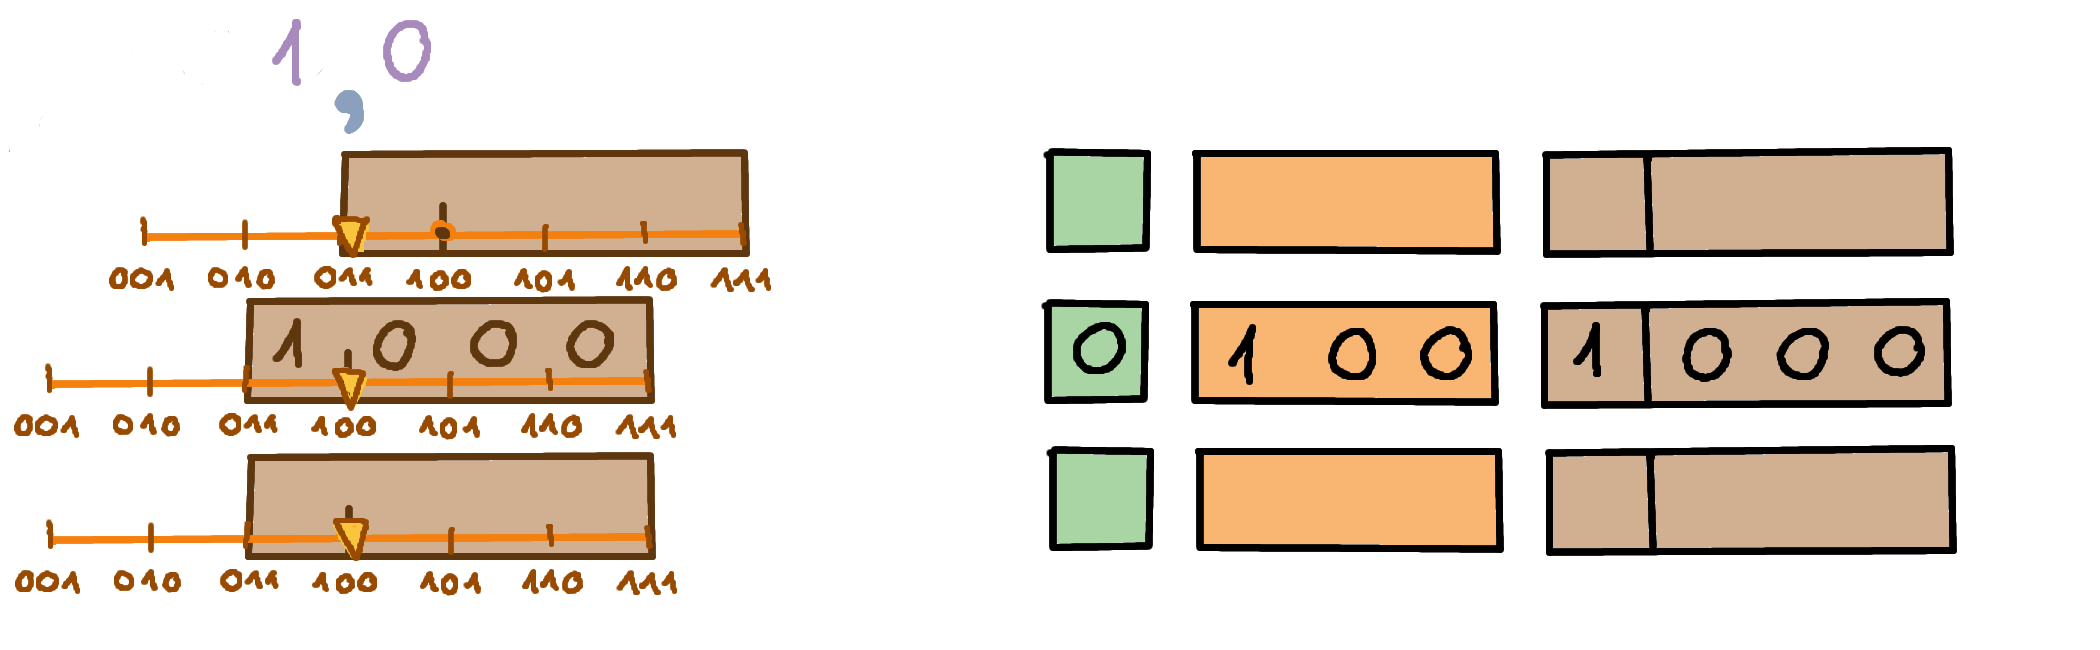
\includegraphics[width=\linewidth]{Pictures/Nachbarn1-4-3.png}
\end{figure}

\item Fülle die vorherige und die nächste darstellbare Zahlen im Fliesskommazahlensystem mit Mantissenlänge \(5\) und Exponent zwischen \(-1\) und \(1\) aus.
\begin{figure}[H]
\centering
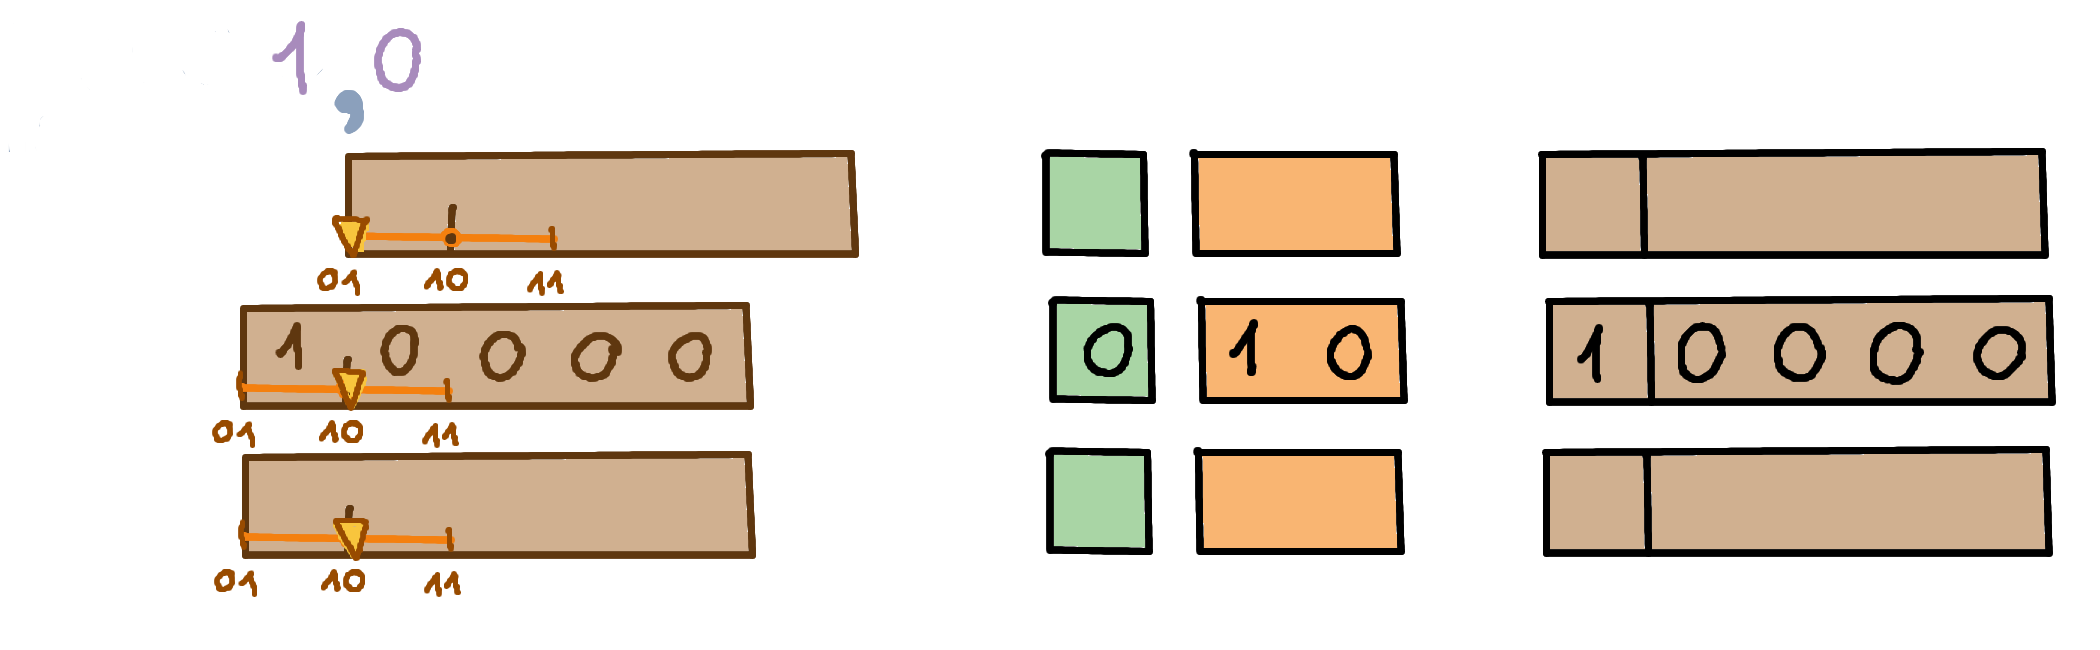
\includegraphics[width=\linewidth]{Pictures/Nachbarn1-5-2.png}
\end{figure}

\item Bei welchem Fliesskommazahlensystem ist der Abstand zwischen benachbarten Zahlen änhlich zu dem im Fliesskommazahlensystem mit Mantissenlänge \(5\) und Exponent zwischen \(-3\) und \(3\)?
\end{enumerate}

\end{aufgabe}

\subsubsection*{\textcolor{blue-violet}{Teste dich selber}}

\begin{aufgabe}\label{fliesskommazahlen_kontrollfragen}
Beantworte folgende Fragen:
\begin{enumerate}[(a)]
\item Kann man im Fliesskommazahlensystem alle reelle Zahlen darstellen? Wieso?
\item Gibt es eine grösste Zahl im Fliesskommazahlensystem? Falls nein, warum? Falls ja, wie findet man sie?
\item Gibt es eine kleinste Zahl im Fliesskommazahlensystem? Falls nein, warum? Falls ja, wie findet man sie?
\item Was beeinflusst stärker den Bereich der positiven darstellbaren Zahlen in einem Fliesskommasystem? Die Mantissenlänge oder die Länge der Exponentenkodierung?
\item Gib eine Zahl zwischen \(1/2\) und \(3.5\) an, die im Fliesskommazahlensystem mit Mantissenlänge \(3\) und Exponenten von \(-1\) bis \(1\) nicht darstellbar ist.
\item Sind alle Zahlen im Fliesskommazahlensystem gleichverteilt? Falls nicht, welche Zahlen stehen dichter beieinander, die kleineren oder die grösseren?
\item Was beeinflusst stärker den Abstand zwischen den positiven darstellbaren Zahlen in einem Fliesskommazahlensystem? Die Mantissenlänge oder die Länge der Exponentenkodierung?
\end{enumerate}
\end{aufgabe}
